%  LaTeX support: latex@mdpi.com 
%  For support, please attach all files needed for compiling as well as the log file, and specify your operating system, LaTeX version, and LaTeX editor.

%=================================================================
\documentclass[sensors,article,submit,pdftex,moreauthors]{Definitions/mdpi} 
% For posting an early version of this manuscript as a preprint, you may use "preprints" as the journal and change "submit" to "accept". The document class line would be, e.g., \documentclass[preprints,article,accept,moreauthors,pdftex]{mdpi}. This is especially recommended for submission to arXiv, where line numbers should be removed before posting. For preprints.org, the editorial staff will make this change immediately prior to posting.

%--------------------
% Class Options:
%--------------------
%----------
% journal
%----------
% Choose between the following MDPI journals:
% acoustics, actuators, addictions, admsci, adolescents, aerospace, agriculture, agriengineering, agronomy, ai, algorithms, allergies, alloys, analytica, animals, antibiotics, antibodies, antioxidants, applbiosci, appliedchem, appliedmath, applmech, applmicrobiol, applnano, applsci, aquacj, architecture, arts, asc, asi, astronomy, atmosphere, atoms, audiolres, automation, axioms, bacteria, batteries, bdcc, behavsci, beverages, biochem, bioengineering, biologics, biology, biomass, biomechanics, biomed, biomedicines, biomedinformatics, biomimetics, biomolecules, biophysica, biosensors, biotech, birds, bloods, blsf, brainsci, breath, buildings, businesses, cancers, carbon, cardiogenetics, catalysts, cells, ceramics, challenges, chemengineering, chemistry, chemosensors, chemproc, children, chips, cimb, civileng, cleantechnol, climate, clinpract, clockssleep, cmd, coasts, coatings, colloids, colorants, commodities, compounds, computation, computers, condensedmatter, conservation, constrmater, cosmetics, covid, crops, cryptography, crystals, csmf, ctn, curroncol, currophthalmol, cyber, dairy, data, dentistry, dermato, dermatopathology, designs, diabetology, diagnostics, dietetics, digital, disabilities, diseases, diversity, dna, drones, dynamics, earth, ebj, ecologies, econometrics, economies, education, ejihpe, electricity, electrochem, electronicmat, electronics, encyclopedia, endocrines, energies, eng, engproc, ent, entomology, entropy, environments, environsciproc, epidemiologia, epigenomes, est, fermentation, fibers, fintech, fire, fishes, fluids, foods, forecasting, forensicsci, forests, foundations, fractalfract, fuels, futureinternet, futureparasites, futurepharmacol, futurephys, futuretransp, galaxies, games, gases, gastroent, gastrointestdisord, gels, genealogy, genes, geographies, geohazards, geomatics, geosciences, geotechnics, geriatrics, hazardousmatters, healthcare, hearts, hemato, heritage, highthroughput, histories, horticulturae, humanities, humans, hydrobiology, hydrogen, hydrology, hygiene, idr, ijerph, ijfs, ijgi, ijms, ijns, ijtm, ijtpp, immuno, informatics, information, infrastructures, inorganics, insects, instruments, inventions, iot, j, jal, jcdd, jcm, jcp, jcs, jdb, jeta, jfb, jfmk, jimaging, jintelligence, jlpea, jmmp, jmp, jmse, jne, jnt, jof, joitmc, jor, journalmedia, jox, jpm, jrfm, jsan, jtaer, jzbg, kidney, kidneydial, knowledge, land, languages, laws, life, liquids, literature, livers, logics, logistics, lubricants, lymphatics, machines, macromol, magnetism, magnetochemistry, make, marinedrugs, materials, materproc, mathematics, mca, measurements, medicina, medicines, medsci, membranes, merits, metabolites, metals, meteorology, methane, metrology, micro, microarrays, microbiolres, micromachines, microorganisms, microplastics, minerals, mining, modelling, molbank, molecules, mps, msf, mti, muscles, nanoenergyadv, nanomanufacturing, nanomaterials, ncrna, network, neuroglia, neurolint, neurosci, nitrogen, notspecified, nri, nursrep, nutraceuticals, nutrients, obesities, oceans, ohbm, onco, oncopathology, optics, oral, organics, organoids, osteology, oxygen, parasites, parasitologia, particles, pathogens, pathophysiology, pediatrrep, pharmaceuticals, pharmaceutics, pharmacoepidemiology, pharmacy, philosophies, photochem, photonics, phycology, physchem, physics, physiologia, plants, plasma, pollutants, polymers, polysaccharides, poultry, powders, preprints, proceedings, processes, prosthesis, proteomes, psf, psych, psychiatryint, psychoactives, publications, quantumrep, quaternary, qubs, radiation, reactions, recycling, regeneration, religions, remotesensing, reports, reprodmed, resources, rheumato, risks, robotics, ruminants, safety, sci, scipharm, seeds, sensors, separations, sexes, signals, sinusitis, skins, smartcities, sna, societies, socsci, software, soilsystems, solar, solids, sports, standards, stats, stresses, surfaces, surgeries, suschem, sustainability, symmetry, synbio, systems, taxonomy, technologies, telecom, test, textiles, thalassrep, thermo, tomography, tourismhosp, toxics, toxins, transplantology, transportation, traumacare, traumas, tropicalmed, universe, urbansci, uro, vaccines, vehicles, venereology, vetsci, vibration, viruses, vision, waste, water, wem, wevj, wind, women, world, youth, zoonoticdis 

%---------
% article
%---------
% The default type of manuscript is "article", but can be replaced by: 
% abstract, addendum, article, book, bookreview, briefreport, casereport, comment, commentary, communication, conferenceproceedings, correction, conferencereport, entry, expressionofconcern, extendedabstract, datadescriptor, editorial, essay, erratum, hypothesis, interestingimage, obituary, opinion, projectreport, reply, retraction, review, perspective, protocol, shortnote, studyprotocol, systematicreview, supfile, technicalnote, viewpoint, guidelines, registeredreport, tutorial
% supfile = supplementary materials

%----------
% submit
%----------
% The class option "submit" will be changed to "accept" by the Editorial Office when the paper is accepted. This will only make changes to the frontpage (e.g., the logo of the journal will get visible), the headings, and the copyright information. Also, line numbering will be removed. Journal info and pagination for accepted papers will also be assigned by the Editorial Office.

%------------------
% moreauthors
%------------------
% If there is only one author the class option oneauthor should be used. Otherwise use the class option moreauthors.

%---------
% pdftex
%---------
% The option pdftex is for use with pdfLaTeX. If eps figures are used, remove the option pdftex and use LaTeX and dvi2pdf.

%=================================================================
% MDPI internal commands
\firstpage{1} 
\makeatletter 
\setcounter{page}{\@firstpage} 
\makeatother
\pubvolume{1}
\issuenum{1}
\articlenumber{0}
\pubyear{2022}
\copyrightyear{2022}
%\externaleditor{Academic Editor: Firstname Lastname}
\datereceived{} 
\dateaccepted{} 
\datepublished{} 
%\datecorrected{} % Corrected papers include a "Corrected: XXX" date in the original paper.
%\dateretracted{} % Corrected papers include a "Retracted: XXX" date in the original paper.
\hreflink{https://doi.org/} % If needed use \linebreak
%\doinum{}
%------------------------------------------------------------------
% The following line should be uncommented if the LaTeX file is uploaded to arXiv.org
%\pdfoutput=1

%=================================================================
% Add packages and commands here. The following packages are loaded in our class file: fontenc, inputenc, calc, indentfirst, fancyhdr, graphicx, epstopdf, lastpage, ifthen, lineno, float, amsmath, setspace, enumitem, mathpazo, booktabs, titlesec, etoolbox, tabto, xcolor, soul, multirow, microtype, tikz, totcount, changepage, attrib, upgreek, cleveref, amsthm, hyphenat, natbib, hyperref, footmisc, url, geometry, newfloat, caption

%=================================================================
%% Please use the following mathematics environments: Theorem, Lemma, Corollary, Proposition, Characterization, Property, Problem, Example, ExamplesandDefinitions, Hypothesis, Remark, Definition, Notation, Assumption
%% For proofs, please use the proof environment (the amsthm package is loaded by the MDPI class).

%=================================================================
% Full title of the paper (Capitalized)
\Title{A Deep Learning Approach for Gait Event Detection from a Single Shank-Worn IMU: Validation in Healthy and Neurological Cohorts}

% MDPI internal command: Title for citation in the left column
\TitleCitation{A Deep Learning Approach for Gait Event Detection from a Single Shank-Worn IMU: Validation in Healthy and Neurological Cohorts}

% Author Orchid ID: enter ID or remove command
\newcommand{\orcidauthorA}{0000-0002-2507-0924} % Add \orcidA{} behind the author's name
%\newcommand{\orcidauthorB}{0000-0000-0000-000X} % Add \orcidB{} behind the author's name

% Authors, for the paper (add full first names)
\Author{Robbin Romijnders$^{1}$\orcidA{}, Elke Warmerdam$^{2}$, Clint Hansen$^{1}$*, Gerhard Schmidt$^{3}$ and Walter Maetzler$^{1,}$}

%\longauthorlist{yes}

% MDPI internal command: Authors, for metadata in PDF
\AuthorNames{Robbin Romijnders, Elke Warmerdam, Clint Hansen, Gerhard Schmidt and Walter Maetzler}

% MDPI internal command: Authors, for citation in the left column
\AuthorCitation{Romijnders, R.; Warmerdam, E.; Hansen, C.; Schmidt, G.; Maetzler, W.}
% If this is a Chicago style journal: Lastname, Firstname, Firstname Lastname, and Firstname Lastname.

% Affiliations / Addresses (Add [1] after \address if there is only one affiliation.)
\address{%
$^{1}$ \quad Department of Neurology, Kiel University, 24105 Kiel, Germany; r.romijnders@neurologie.uni-kiel.de (R.R.), c.hansen@neurologie.uni-kiel.de (C.H.), w.maetzler@neurologie.uni-kiel.de (W.M.)\\
$^{2}$ \quad xxxxx, xxxxx, xxxxx Homburg, Germany; elke.warmerdam@uni-saarland.de (E.W.)\\
$^{3}$ \quad Institute of Electrical Engineering and Information Technology, Faculty of Engineering, Kiel University, 24143 Kiel, Germany; gus@tf.uni-kiel.de (G.S.)}

% Contact information of the corresponding author
\corres{Correspondence: r.romijnders@neurologie.uni-kiel.de (R.R.)}

% Current address and/or shared authorship
%\firstnote{Current address: Affiliation 3.} 
%\secondnote{These authors contributed equally to this work.}
% The commands \thirdnote{} till \eighthnote{} are available for further notes

%\simplesumm{} % Simple summary

%\conference{} % An extended version of a conference paper

% Abstract (Do not insert blank lines, i.e. \\) 
\abstract{A single paragraph of about 200 words maximum. For research articles, abstracts should give a pertinent overview of the work. We strongly encourage authors to use the following style of structured abstracts, but without headings: (1) Background: place the question addressed in a broad context and highlight the purpose of the study; (2) Methods: describe briefly the main methods or treatments applied; (3) Results: summarize the article's main findings; (4) Conclusions: indicate the main conclusions or interpretations. The abstract should be an objective representation of the article, it must not contain results which are not presented and substantiated in the main text and should not exaggerate the main conclusions.}

% Keywords
\keyword{keyword 1; keyword 2; keyword 3 (List three to ten pertinent keywords specific to the article; yet reasonably common within the subject discipline.)} 

% The fields PACS, MSC, and JEL may be left empty or commented out if not applicable
%\PACS{J0101}
%\MSC{}
%\JEL{}

%%%%%%%%%%%%%%%%%%%%%%%%%%%%%%%%%%%%%%%%%%
% Only for the journal Diversity
%\LSID{\url{http://}}

%%%%%%%%%%%%%%%%%%%%%%%%%%%%%%%%%%%%%%%%%%
% Only for the journal Applied Sciences:
%\featuredapplication{Authors are encouraged to provide a concise description of the specific application or a potential application of the work. This section is not mandatory.}
%%%%%%%%%%%%%%%%%%%%%%%%%%%%%%%%%%%%%%%%%%

%%%%%%%%%%%%%%%%%%%%%%%%%%%%%%%%%%%%%%%%%%
% Only for the journal Data:
%\dataset{DOI number or link to the deposited data set in cases where the data set is published or set to be published separately. If the data set is submitted and will be published as a supplement to this paper in the journal Data, this field will be filled by the editors of the journal. In this case, please make sure to submit the data set as a supplement when entering your manuscript into our manuscript editorial system.}

%\datasetlicense{license under which the data set is made available (CC0, CC-BY, CC-BY-SA, CC-BY-NC, etc.)}

%%%%%%%%%%%%%%%%%%%%%%%%%%%%%%%%%%%%%%%%%%
% Only for the journal Toxins
%\keycontribution{The breakthroughs or highlights of the manuscript. Authors can write one or two sentences to describe the most important part of the paper.}

%%%%%%%%%%%%%%%%%%%%%%%%%%%%%%%%%%%%%%%%%%
% Only for the journal Encyclopedia
%\encyclopediadef{Instead of the abstract}
%\entrylink{The Link to this entry published on the encyclopedia platform.}
%%%%%%%%%%%%%%%%%%%%%%%%%%%%%%%%%%%%%%%%%%
\begin{document}

%%%%%%%%%%%%%%%%%%%%%%%%%%%%%%%%%%%%%%%%%%
\section{Introduction}
Gait deficits are common in older adults and possibly reflect the presence of an underlying neurodegenerative disease \cite{Snijders2007,Hodgins2008}. For example, conversion to Parkinson's Disease \cite{DelDin2019} or from mild cognitive impairment to Alzheimer's Disease \cite{Koenig2017,Bertoli2018} are linked with changes in spatiotemporal gait parameters. Similarly, temporal gait parameters are different for stroke patients \cite{SchroederVon1995,Mohan2021} and patients with multiple sclerosis \cite{Griskevicius2016,Flachenecker2019} when compared to healthy controls. To objectively quantify gait deficits, stride-specific parameters such as stride time or stride length are often used \cite{Hannink2016}, where the beginning and end of a stride are determined from two successive initial contacts (ICs) of the same foot \cite{Perry2010,Whittle2012}. The IC is when the foot contacts the ground and together with the instant at which the foot leaves the ground (final contact, FC), each stride can be divided in a stance and swing phase \cite{Rueterbories2010,Bruening2014}.  The events of IC and FC, also referred to as \emph{gait events}, are commonly determined using force or pressure measuring devices \cite{Bruening2014}, or stereophotogrammetry systems based on reflective markers using a multi-camera setup \cite{Chiari2005}. These systems are relatively expensive, and restricted to usage in expertise laboratories \cite{Iosa2016,Jarchi2018}. As there is increasing evidence that gait measured in the lab does not reflect daily-life gait \cite{Hillel2019,Warmerdam2020,Atrsaei2021}, there is more and more interest in measurement systems that allow for continuous gait analysis in ambulatory settings. Therefore, the use of inertial measurement units (IMUs) is especially attractive, as these can be used to measure gait in ecologically valid environments, such as the home environment, thereby painting a more complete picture of health status \cite{DelDin2016,Shah2020} and providing clinical information that is complementary to standardized lab-based assessments \cite{Warmerdam2020,Fasano2020,Atrsaei2021,Corra2021}.

Previous research suggests that gait event detection is more accurate using an IMU worn on a lower limb (e.g., shank or foot) compared to an IMU worn on the low back \cite{BenMansour2015,Storm2016,Panebianco2018}. Now, in order to get from abstract IMU sensor readings to clinically relevant gait parameters (e.g., from accelerations and angular velocities to stride times) \cite{Hannink2016}, different algorithmic approaches have been developed in the last twenty years of clinical gait research. A recent study has evaluated a cross-section of these algorithms for different sensor locations on the lower leg and foot \cite{Niswander2021}. The algorithms were categorized according to which signals were analyzed, for example the angular velocity about the medio-lateral axis, or the accelerations along vertical and antero-posterior axis. This means the sensor readings need to be linked with the anatomical axes, that is, one needs to know which sensor axis aligns with for example the medio-lateral axis. In most approaches, it is simply assumed that due to sensor attachment the sensor axis aligns roughly with the anatomical axis of interest (\cite{Salarian2004,Sabatini2005,Jasiewicz2006,Catalfamo2010,Trojaniello2014,Maqbool2016,Romijnders2021}) or an additional calibration procedure (e.g., \cite{Ferraris1995}) is required (\cite{Greene2010,Niswander2021}). In ambulatory assessments however, study participants often attach the sensor themselves, and therefore the sensor location and alignment cannot be controlled for. Furthermore, it is unlikely that each time the sensor is (re-)attached study participants, especially those with gait deficits, perform a calibration procedure that usually consists of holding a pre-defined pose and performing some known movement sequences (TODO: reference?! Kong? Seel?). 

Taken together, this drives the need for an approach that is invariant to sensor orientation, and is applicable across a variety of pathological gait patterns. As pointed out by \cite{Hannink2016}, in the field of image analysis similar requirements have been successfully addressed by algorithms that share a common underlying methodology referred to as deep learning \cite{LeCun2015,TerHaarRomeny2019}. Recent applications of deep learning algorithms have already shown improved performance in detecting gait events from marker-based motion capture when compared to conventional, often heuristics-based, algorithms \cite{Kidzinski2019,Lempereur2020,Filtjens2020}. Another study used a deep learning approach to detect gait events from either three IMUs (worn on the low back, and both ankles) or a single IMU (worn on the low back), and showed that the time error was considerably smaller for the deep learning algorithm than for a commonly applied wavelet-based approach \cite{Gadaleta2019}.

In this study, we further these works by validating this deep learning approach for detecting gait events in a heterogeneous cohort of healthy and neurologically diseased adults considering a single IMU setup, worn on the lower leg.
%%%%%%%%%%%%%%%%%%%%%%%%%%%%%%%%%%%%%%%%%%
\section{Materials and Methods}

\subsection{Data Collection}
Gait analyses were performed in the Universit\"{a}tsklinikum Schleswig-Holstein (UKSH) campus Kiel, Germany. The study \cite{Warmerdam2021} was approved by the ethical committee of the medical faculty at the UKSH (no: D438/18). In total, data from 160 participants were included for the current analysis, including data from young adults (YA; age: 18 - 60 years), older adults (OA; age: $>$60 years), people with Parkinson's Disease (PD; according to the UK Brain Bank criteria \cite{Gibb1988}), people with a recent ($<$4 weeks) symptomatic stroke (stroke), people with multiple sclerosis (MS; according to the McDonalds criteria \cite{Thompson2018}), people with chronic low back pain (cLBP), and people with other diagnoses that were assumed not to affect mobility (Table \ref{tab:demographics_data}). Inclusion criteria were an age of 18 years or older, and the ability to walk independently without a walking aid. Participants were excluded from the study with a Montreal Cognitive Assessment \cite{Nasreddine2005} score $<$15 and other movement disorders that affected mobility, as noticed by the clinical assessor.

\begin{table}[H] 
	\caption{\label{tab:demographics_data}Demographics data of the study participants. Age, height, and weight are presented as mean (standard deviation).}
	\newcolumntype{C}{>{\centering\arraybackslash}X}
	\begin{tabularx}{\textwidth}{CCCCCC}
		\toprule
		\textbf{Group}	& \textbf{Gender}	& \textbf{Number of}	& \textbf{Age}	& \textbf{Height}	& \textbf{Weight}\\
		 & & \textbf{subjects} & years	& cm	& kg\\
		\midrule
		YA		& F		& 21	& 27 (7)	& 173 (5)	& 67 (8)\\
		 & M	& 22	& 30 (9)	& 185 (8) & 81 (13)\\ 
		\midrule
		OA		& F		& 11	& 70 (6)	& 167 (6)	& 72 (17)\\
		 & M	& 11	& 73 (6)	& 180 (6) & 83 (11)\\
		\midrule
		PD		& F		& 12	& 67 (6)	& 168 (6)	& 70 (14)\\
		 & M	& 20	& 62 (11)	& 178 (6) & 87 (13)\\
		\midrule
		MS		& F		& 12	& 37 (9)	& 174 (9)	& 75 (9)\\
		 & M	& 9	& 42 (15)	& 189 (8) & 96 (30)\\
		\midrule
		stroke	& F		& 4	& 66 (10)	& 160 (6)	& 65 (11)\\
		 & M	& 17	& 67 (17)	& 178 (7) & 84 (14)\\
		\midrule
		cLBP	& F		& 3	& 64 (10)	& 166 (5)	& 65 (5)\\
		 & M	& 7	& 63 (16)	& 178 (7) & 90 (16)\\ 
		\midrule
		other	& F		& 3	& 60 (13)	& 166 (3)	& 79 (15)\\
		 & M	& 8	& 68 (18)	& 182 (7) & 85 (13)\\ 
		\bottomrule
	\end{tabularx}
	\noindent{\footnotesize{\textbf{Group}: YA: younger adults, OA: older adults, PD: Parkinson's Disease, MS: multiple sclerosis, cLBP: chronic low back pain; \textbf{Gender}: F: female, M: male.}}
\end{table}

Participants performed three walking trials consisting of walking 5 meter at either (1) preferred speed ("\emph{Please walk at your normal walking speed.}"), (2) slow speed ("\emph{Please walk half of your normal walking speed.}"), or (3) fast speed ("\emph{Please walk as fast as possible, without running or falling.}"). The 5 meter distance was marked with two cones on both ends, and participants were asked to start walking approximately two steps before the cones on one end, and stop walking approximately two steps after passing the cones on the other end.

For the current analysis data from four IMUs (Noraxon USA Inc., myoMOTION, Scottsdale, AZ, USA) were considered, namely those that were attached laterally above the left and right ankle joint and those attached proximally at the left and right shank. IMUs were secured to participants using elastic bands with a special hold for the IMU. Furthermore, reflective markers were attached on top of the usual foot wear at the heel and toe of both feet. Marker data were recorded using a twelve-camera stereophotogrammetry system (Qualisys AB, G\"{o}teborg, Sweden) at a sampling frequency of 200 Hz. IMU data were recorded at the same sampling frequency, and both systems were synchronized using TTL signal \cite{Warmerdam2021}. For some recordings, the sampling frequency of the IMUs was erroneously set at 100 Hz, and therefore data from these trials were upsampled before further analysis.

\subsection{Data Pre-processing \label{subsec:data_preprocessing}}
\subsubsection{Reference Values}
The raw reflective marker data were first used to determine the start and end of each trial. The start of the trial was defined as the time for which the first toe marker (left or right) crossed the \emph{virtual} starting line. The end was defined as the time for which the last heel marker crossed the end line. For both marker and IMU systems, data were then cropped from start to the end of the trial.

Any remaining gaps in the marker data were filled by interpolation making use of inter-correlations between markers \cite{Federolf2013,Gloersen2016}. The data were then low-pass filtered using a double pass 6th order Butterworth filter with a cut-off frequency of 20 Hz \cite{Kormylo1974,Racz2021}. The filtered data were differentiated to get velocity signals, and timings of ICs and FCs were determined from local maxima and minima in the heel and toe vertical velocity signals \cite{Pijnappels2001,OConnor2007}. Like in \cite{Carcreff2018,Romijnders2021}, all identified ICs and FCs were manually checked using Qualisys Track Manager 2018.1 software (QTM; Qualisys AB, Göteborg, Sweden).

\subsubsection{IMU Data}
For the deep learning model, the data from randomly selected one-third of participants were used as a "training set", another one-third was used as a "validation set", and the rest was used as "test set", where randomization was stratified by both group and gender. Accelerometer and gyroscope data from the four IMUs were normalized by subtracting the channel-wise mean, and dividing by the channel-wise standard deviation. Then, for the training and validation set, the time series data were partitioned into equal length time windows of 400 samples, with an overlap of 50\% between successive windows.


\subsection{Model}
\subsubsection{Notation}
Data from the IMUs' 3D accelerometer and 3D gyroscope were used. A signal was considered a sequence of real-valued numbers: $\mathbf{x} = \begin{array}{ccccc}
	\cdots & x[n-1] & x[n] & x[n+1] & \cdots
\end{array}$, with $n = 1, \cdots, N$ the discrete-time sample index. For any given channel, e.g., acceleration in $X$-direction, the signal was denoted in vector notation as: $\mathbf{x}_{d} = \begin{bmatrix}
x_{d}[1] & x_{d}[2] & \cdots & x_{d}[N]
\end{bmatrix}^{\mathrm{T}}$, where $d$ referred to the $d$-th channel.

Data from all channels of a single IMU were collected in a $ N \times D$ data matrix, like:
\begin{equation}
	\mathbf{X} = \begin{bmatrix}
		\vdots & \vdots &  & \vdots\\
		\mathbf{x}_{1} & \mathbf{x}_{2} & \cdots & \mathbf{x}_{D}\\
		\vdots & \vdots &  & \vdots
	\end{bmatrix} = \begin{bmatrix}
		x_{1}[1] & x_{2}[1] & & x_{D}[1]\\
		x_{1}[2] & x_{2}[2] & & x_{D}[2]\\
		\vdots & \vdots & \cdots & \vdots\\
		x_{1}[N] & x_{2}[1] & & x_{D}[N]\end{bmatrix}, \quad \mathbf{X} \in \mathbb{R}^{N \times D}
	\label{eqn:train_data_single_instance}
\end{equation}

The corresponding labels (or targets) were then denoted as:
\begin{equation}
	\mathbf{y}_{\mathrm{IC}} = \begin{bmatrix}
		y_{1}[1]\\
		y_{1}[2]\\
		\vdots\\
		y_{1}[N]
	\end{bmatrix}, \quad \mathbf{y}_{\mathrm{FC}} = \begin{bmatrix}
		y_{2}[1]\\
		y_{2}[2]\\
		\vdots\\
		y_{2}[N]
	\end{bmatrix}, \quad y_{i}[n] \in [0, 1]
	\label{eqn:train_labels_single_instace}
\end{equation}


\subsubsection{Model Architecture}
The basic architecture for the deep learning model was a temporal convolutional network (TCN) \cite{Bai2018,Remy2020,Filtjens2020}. The TCN consisted of repeating blocks of dilated convolutions (CONV) \cite{YuKoltun2016,Bai2018} that were followed by batch normalization (BN) \cite{Ioffe2015}, rectified linear unit (ReLU) activation, and dropout (DropOut) \cite{Srivastava2014}. For each given dilation factor, the sequence of layers CONV-BN-ReLU-DropOut was repeated twice \cite{Remy2020}. Dilation factors were given as a sequence of increasing powers of 2, e.g., $\left\{1, 2, 4, 8\right\}$ \cite{VanDenOord2016,YuKoltun2016,Bai2018}. These repeating blocks were followed by a fully-connected (dense) layer with sigmoid activation, and outputs were predicted separately for ICs and FCs. The mean squared error (MSE) was used as loss function, and a gradient descent-based optimization algorithm with adaptive moment (Adam) optimizer was used to iteratively learn the weights \cite{Kingma2014,Schmidt2021}.

\subsubsection{Hyperparameter Optimization}
In order to find the best model architecture, hyperparameter tuning was perfomed using KerasTuner \cite{OMalley2019}. Here, the number of filters, the kernel size, and the maximum dilation factor (Table \ref{tab:hyperparameter_optimization}) were optimized for using a random search strategy \cite{Bergstra2012}.

\begin{table}[H] 
	\caption{Model hyperparameters that were optimized for, and the corresponding sets of possible values.\label{tab:hyperparameter_optimization}}
	\newcolumntype{C}{>{\centering\arraybackslash}X}
	\begin{tabularx}{\textwidth}{CC}
		\toprule
		\textbf{Description}	& \textbf{Possible values}\\
		\midrule
		Number of filters	& 8, 16, 32, 64, 128\\
		Kernel size			& 3, 5, 7\\
		Dilations 			& [1, 2], [1, 2, 4], [1, 2, 4, 8]\\
		\bottomrule
	\end{tabularx}
\end{table}

The model architecture that resulted from the hyperparameter optimization was then trained on the combined set of training and validation data. The trained model was used to predict occurrence of gait events from the hold-out test set.

\subsection{Analysis}
The predictions of the model on the test set data were compared with the labels from the test set. The model performance was evaluated for (1) overall detection performance, (2) time agreement between the predicted events and the (marker-based) annotated events, (3) agreement between subsequently derived gait parameters.
\subsubsection{Overall detection performance \label{subsubsec:overall_detection_performance}}
The overall detection performance quantified how many of the annotated evens were detected by the model (true positives, TP), how many of the annotated events were not detected (false negatives, FN), and how many event that were detected, were actually not annotated (false positives, FP). From these metrics, the recall (or sensitivity), precision and F$_{1}$ score were calculated as:
\begin{equation}
	\textrm{recall} = \frac{\textrm{TP}}{\textrm{TP} + \textrm{FN}} \nonumber
	\label{eqn:recall}
\end{equation}
\begin{equation}
	\textrm{precision} = \frac{\textrm{TP}}{\textrm{TP} + \textrm{FP}} \nonumber
	\label{eqn:precision}
\end{equation}
\begin{equation}
	\textrm{F$_{1}$ score} = 2 \cdot \frac{\textrm{recall} \cdot \textrm{precision}}{\textrm{recall} + \textrm{precision}}  \nonumber
	\label{eqn:f1_score}
\end{equation}

\subsubsection{Time agreement}
For all correctly detected gait events (TP, Section \ref{subsubsec:overall_detection_performance}), the time error between the annotated and detect gait event was defined as:
\begin{equation}
	\textrm{time error} = t_{\textrm{ref}} - t_{\textrm{pred}}
	\label{eqn:time_agreement}
\end{equation}
with $t_{\mathrm{ref}}$ the gait event time from the marker-based annotations, and $t_{\mathrm{pred}}$ the gait event time from the model predictions. As a robust measure for the average time error and its spread, the median time error and the inter-quartile range (IQR) were reported \cite{OpenIntro2019}.

\subsubsection{Gait parameters}
For those trials for which all gait events were detected, and no spurious events were detected, the following stride parameters were calculated:
\begin{equation}
	\textrm{stride time} = t_{\textrm{IC}_{k}} - t_{\textrm{IC}_{k-1}}
	\label{eqn:stride_time}
\end{equation}
\begin{equation}
	\textrm{stance time} = t_{\textrm{FC}_{k}} - t_{\textrm{IC}_{k-1}}
	\label{eqn:stance_time}
\end{equation}
\begin{equation}
	\textrm{swing time} = t_{\textrm{IC}_{k}} - t_{\textrm{FC}_{k}}
	\label{eqn:swing_time}
\end{equation}

%%%%%%%%%%%%%%%%%%%%%%%%%%%%%%%%%%%%%%%%%%
\section{Results}

\subsection{Overall detection performance}
The performance of detecting initial contacts and final contacts was objectively quantified by the number of annotated events that were detected (true positives, TP), the number of annotated events that were not detected (false negatives, FN), and the number of detected events that were not annotated (false positives, FP). From these, recall, precision and F$_{1}$ score were calculated (Table \ref{tab:overall_detection_performance}).
\begin{table}[H]
	\caption{Overall detection performance for initial contacts and final contacts as quantified by recall, precision and F$_{1}$ score.\label{tab:overall_detection_performance}}
	\begin{adjustwidth}{-\extralength}{0cm}
		\newcolumntype{C}{>{\centering\arraybackslash}X}
		\begin{tabularx}{\fulllength}{r|CCCCCC|CCCCCC}
			\toprule
			 & \multicolumn{6}{c}{\textbf{Initial contacts}}	& \multicolumn{6}{c}{\textbf{Final contacts}}\\
			\textbf{Tracked point}	& \textbf{TP}	& \textbf{FN}	& \textbf{FP}	& \textbf{recall}	& \textbf{precision}	& \textbf{F1}	& \textbf{TP}	& \textbf{FN}	& \textbf{FP}	& \textbf{recall}	& \textbf{precision} 	& \textbf{F1}\\
			\midrule
			left ankle		& 624	& 19	& 5		& 97\%	& 99\%	& 98\%		& 606	& 32	& 10	& 95\%	& 98\%	& 97\%\\
			right ankle		& 599	& 42	& 8 	& 93\%	& 99\%	& 96\%		& 614	& 17	& 12	& 97\%	& 98\%	& 98\%\\
			left shank		& 605	& 38	& 15	& 94\%	& 98\%	& 96\%		& 585	& 53	& 18	& 92\%	& 97\%	& 94\%\\
			right shank		& 603	& 36	& 15 	& 94\%	& 98\%	& 96\%		& 595	& 30	& 9		& 95\%	& 99\%	& 97\%\\
			\bottomrule
		\end{tabularx}
	\end{adjustwidth}
	\noindent{\footnotesize{TP: true positives, FN: false negatives, FP: false positives, F1: F$_{1}$ score.}}
\end{table}

For both ICs and FCs, recall is high for each of the tracked points (i.e, $\ge 92\%$), and so is precision (i.e, $\ge 97\%$). Differences between the tracked points are small, i.e. the minimum recall is $92\%$ and the maximum recall is $97\%$, and the minimum precision is $97\%$ and the maximum precision is $99\%$.


\subsection{Time error}
\begin{figure}[H]
	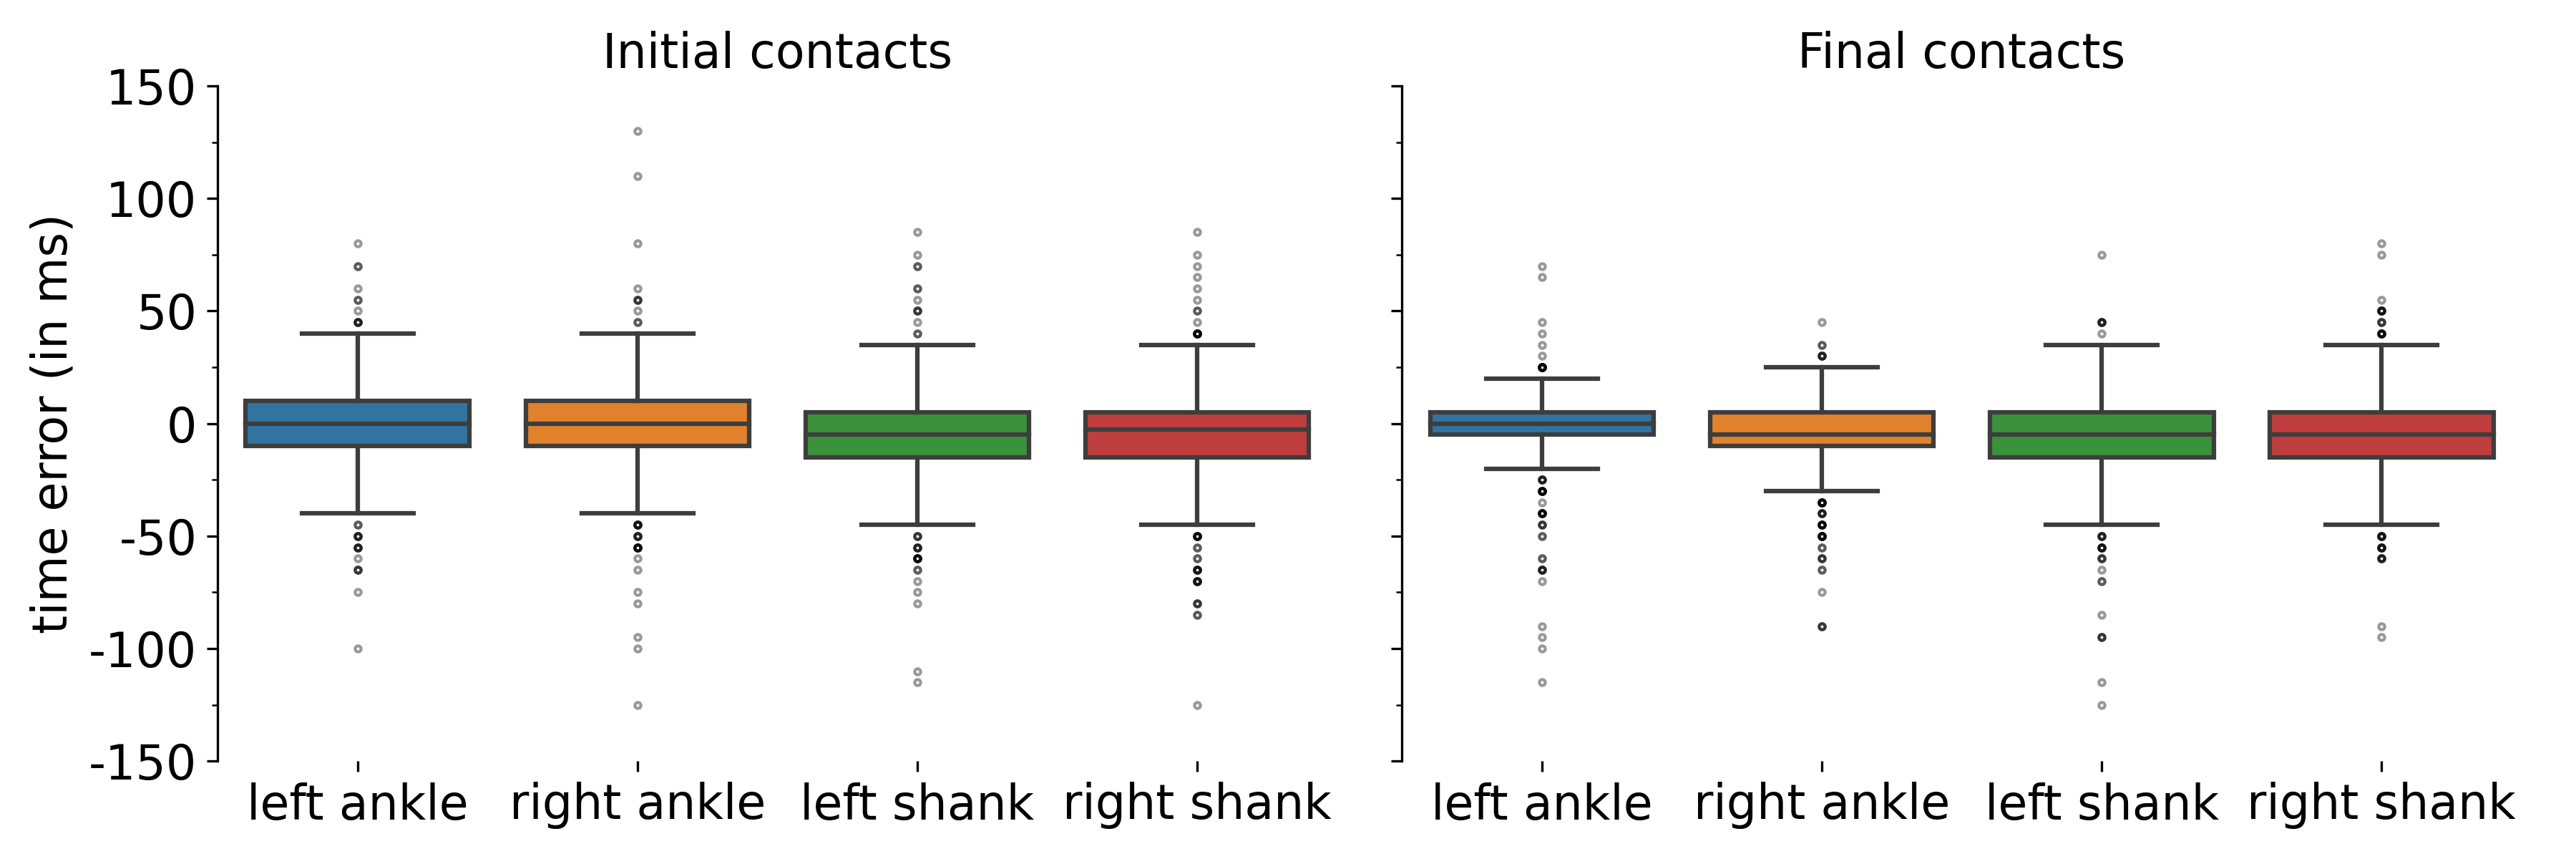
\includegraphics[width=10.5 cm]{fig/box_plots_tracked_points_with_outliers.png}
	\caption{Time errors for initial (left) and final (right) contacts detection, for each of the different tracked points.\label{fig:time_error_box_plots}}
\end{figure}

Time errors for ICs and FCs are visually depicted using boxplots for each tracked point. Data were not normally distributed, thus Wilcoxon signed-rank tests were used to evaluate whether the median time error was zero.
\begin{table}[H] 
	\caption{Time errors for the correctly detected gait events. \label{tab:time_errors}}
	\newcolumntype{C}{>{\centering\arraybackslash}X}
	\begin{tabularx}{\textwidth}{r|CCC|CCC}
		\toprule
		 & \multicolumn{3}{c}{\textbf{Initial contacts}} & \multicolumn{3}{c}{\textbf{Final contacts}}\\
		\textbf{Tracked point} & \textbf{median} & \textbf{IQR} & (\textbf{Q25}, \textbf{Q75}) & \textbf{median} & \textbf{IQR} & (\textbf{Q25}, \textbf{Q75})\\
		 & ms & ms &  (ms, ms) & ms & ms & (ms, ms)\\
		\midrule
		left ankle & 0 & 20 & (-10, 10) & 0 & 10 & (-5, 5)\\
		right ankle & 0 & 20 & (-15, 5) & -5 & 15 & (-10, 5)\\
		left shank & -5 & 20 & (-10, 10) & -5 & 20 & (-15, 5)\\
		right shank & -2.5 & 20 & (-15, 5) & -5 & 20 & (-15, 5)\\
		\bottomrule
	\end{tabularx}
	\noindent{\footnotesize{IQR: inter-quartile range, Q25: 25th percentile, Q75: 75th percentile.}}
\end{table}

\subsection{Gait parameters}
\begin{figure}[H]
	\begin{adjustwidth}{-\extralength}{0cm}
		\centering
		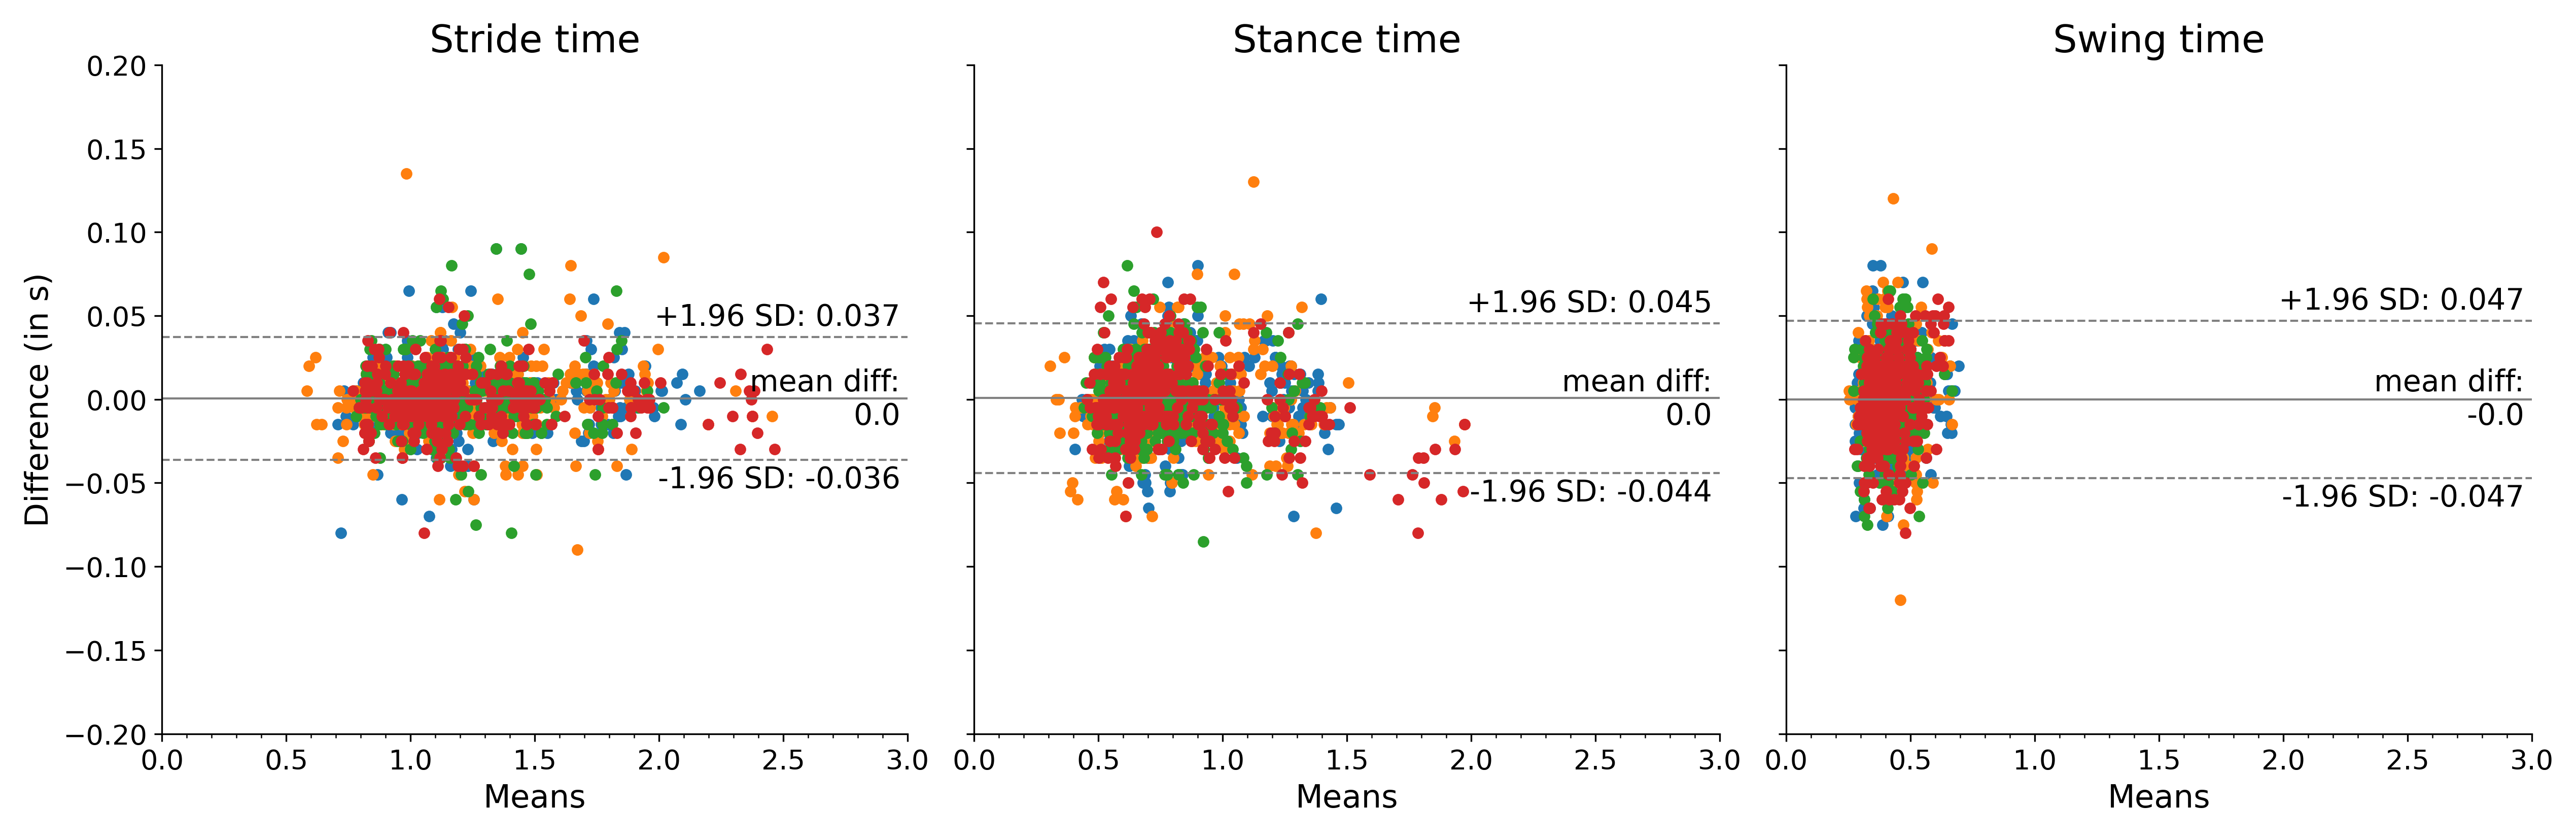
\includegraphics[width=13.5cm]{fig/bland_altman_plots_stride_params.png}
	\end{adjustwidth}
	\caption{The agreement of extracted gait parameters between the sensor-based and marker-based methods.\label{fig:gait_parameters_bland_altman_plots}}
\end{figure}  


This section may be divided by subheadings. It should provide a concise and precise description of the experimental results, their interpretation as well as the experimental conclusions that can be drawn.
\subsection{Subsection}
\subsubsection{Subsubsection}

Bulleted lists look like this:
\begin{itemize}
\item	First bullet;
\item	Second bullet;
\item	Third bullet.
\end{itemize}

Numbered lists can be added as follows:
\begin{enumerate}
\item	First item; 
\item	Second item;
\item	Third item.
\end{enumerate}

The text continues here. 

\subsection{Figures, Tables and Schemes}

All figures and tables should be cited in the main text as Figure~\ref{fig1}, Table~\ref{tab1}, Table~\ref{tab2}, etc.

\begin{figure}[H]

\includegraphics[width=10.5 cm]{Definitions/logo-mdpi}
\caption{This is a figure. Schemes follow the same formatting. If there are multiple panels, they should be listed as: (\textbf{a}) Description of what is contained in the first panel. (\textbf{b}) Description of what is contained in the second panel. Figures should be placed in the main text near to the first time they are cited. A caption on a single line should be centered.\label{fig1}}
\end{figure}   
\unskip

\begin{table}[H] 
\caption{This is a table caption. Tables should be placed in the main text near to the first time they are~cited.\label{tab1}}
\newcolumntype{C}{>{\centering\arraybackslash}X}
\begin{tabularx}{\textwidth}{CCC}
\toprule
\textbf{Title 1}	& \textbf{Title 2}	& \textbf{Title 3}\\
\midrule
Entry 1		& Data			& Data\\
Entry 2		& Data			& Data\\
\bottomrule
\end{tabularx}
\end{table}
\unskip

\begin{table}[H]
\caption{This is a wide table.\label{tab2}}
	\begin{adjustwidth}{-\extralength}{0cm}
		\newcolumntype{C}{>{\centering\arraybackslash}X}
		\begin{tabularx}{\fulllength}{CCCC}
			\toprule
			\textbf{Title 1}	& \textbf{Title 2}	& \textbf{Title 3}     & \textbf{Title 4}\\
			\midrule
			Entry 1		& Data			& Data			& Data\\
			Entry 2		& Data			& Data			& Data \textsuperscript{1}\\
			\bottomrule
		\end{tabularx}
	\end{adjustwidth}
	\noindent{\footnotesize{\textsuperscript{1} This is a table footnote.}}
\end{table}

%\begin{listing}[H]
%\caption{Title of the listing}
%\rule{\columnwidth}{1pt}
%\raggedright Text of the listing. In font size footnotesize, small, or normalsize. Preferred format: left aligned and single spaced. Preferred border format: top border line and bottom border line.
%\rule{\columnwidth}{1pt}
%\end{listing}

Text.

Text.

\subsection{Formatting of Mathematical Components}

This is the example 1 of equation:
\begin{linenomath}
\begin{equation}
a = 1,
\end{equation}
\end{linenomath}
the text following an equation need not be a new paragraph. Please punctuate equations as regular text.
%% If the documentclass option "submit" is chosen, please insert a blank line before and after any math environment (equation and eqnarray environments). This ensures correct linenumbering. The blank line should be removed when the documentclass option is changed to "accept" because the text following an equation should not be a new paragraph.

This is the example 2 of equation:
\begin{adjustwidth}{-\extralength}{0cm}
\begin{equation}
a = b + c + d + e + f + g + h + i + j + k + l + m + n + o + p + q + r + s + t + u + v + w + x + y + z
\end{equation}
\end{adjustwidth}

% Example of a page in landscape format (with table and table footnote).
%\startlandscape
%\begin{table}[H] %% Table in wide page
%\caption{This is a very wide table.\label{tab3}}
%	\begin{tabularx}{\textwidth}{CCCC}
%		\toprule
%		\textbf{Title 1}	& \textbf{Title 2}	& \textbf{Title 3}	& \textbf{Title 4}\\
%		\midrule
%		Entry 1		& Data			& Data			& This cell has some longer content that runs over two lines.\\
%		Entry 2		& Data			& Data			& Data\textsuperscript{1}\\
%		\bottomrule
%	\end{tabularx}
%	\begin{adjustwidth}{+\extralength}{0cm}
%		\noindent\footnotesize{\textsuperscript{1} This is a table footnote.}
%	\end{adjustwidth}
%\end{table}
%\finishlandscape

% Example of a figure that spans the whole page width. The same concept works for tables, too.
\begin{figure}[H]
\begin{adjustwidth}{-\extralength}{0cm}
\centering

\includegraphics[width=13.5cm]{Definitions/logo-mdpi}
\end{adjustwidth}
\caption{This is a wide figure.\label{fig2}}
\end{figure}  

Please punctuate equations as regular text. Theorem-type environments (including propositions, lemmas, corollaries etc.) can be formatted as follows:
%% Example of a theorem:
\begin{Theorem}
Example text of a theorem.
\end{Theorem}

The text continues here. Proofs must be formatted as follows:

%% Example of a proof:
\begin{proof}[Proof of Theorem 1]
Text of the proof. Note that the phrase ``of Theorem 1'' is optional if it is clear which theorem is being referred to.
\end{proof}
The text continues here.

%%%%%%%%%%%%%%%%%%%%%%%%%%%%%%%%%%%%%%%%%%
\section{Discussion}

Authors should discuss the results and how they can be interpreted from the perspective of previous studies and of the working hypotheses. The findings and their implications should be discussed in the broadest context possible. Future research directions may also be highlighted.

%%%%%%%%%%%%%%%%%%%%%%%%%%%%%%%%%%%%%%%%%%
\section{Conclusions}

This section is not mandatory, but can be added to the manuscript if the discussion is unusually long or complex.

%%%%%%%%%%%%%%%%%%%%%%%%%%%%%%%%%%%%%%%%%%
\section{Patents}

This section is not mandatory, but may be added if there are patents resulting from the work reported in this manuscript.

%%%%%%%%%%%%%%%%%%%%%%%%%%%%%%%%%%%%%%%%%%
\vspace{6pt} 

%%%%%%%%%%%%%%%%%%%%%%%%%%%%%%%%%%%%%%%%%%
%% optional
%\supplementary{The following supporting information can be downloaded at:  \linksupplementary{s1}, Figure S1: title; Table S1: title; Video S1: title.}

% Only for the journal Methods and Protocols:
% If you wish to submit a video article, please do so with any other supplementary material.
% \supplementary{The following supporting information can be downloaded at: \linksupplementary{s1}, Figure S1: title; Table S1: title; Video S1: title. A supporting video article is available at doi: link.}

%%%%%%%%%%%%%%%%%%%%%%%%%%%%%%%%%%%%%%%%%%
\authorcontributions{For research articles with several authors, a short paragraph specifying their individual contributions must be provided. The following statements should be used ``Conceptualization, X.X. and Y.Y.; methodology, X.X.; software, X.X.; validation, X.X., Y.Y. and Z.Z.; formal analysis, X.X.; investigation, X.X.; resources, X.X.; data curation, X.X.; writing---original draft preparation, X.X.; writing---review and editing, X.X.; visualization, X.X.; supervision, X.X.; project administration, X.X.; funding acquisition, Y.Y. All authors have read and agreed to the published version of the manuscript.'', please turn to the  \href{http://img.mdpi.org/data/contributor-role-instruction.pdf}{CRediT taxonomy} for the term explanation. Authorship must be limited to those who have contributed substantially to the work~reported.}

\funding{Please add: ``This research received no external funding'' or ``This research was funded by NAME OF FUNDER grant number XXX.'' and  and ``The APC was funded by XXX''. Check carefully that the details given are accurate and use the standard spelling of funding agency names at \url{https://search.crossref.org/funding}, any errors may affect your future funding.}

\institutionalreview{In this section, you should add the Institutional Review Board Statement and approval number, if relevant to your study. You might choose to exclude this statement if the study did not require ethical approval. Please note that the Editorial Office might ask you for further information. Please add “The study was conducted in accordance with the Declaration of Helsinki, and approved by the Institutional Review Board (or Ethics Committee) of NAME OF INSTITUTE (protocol code XXX and date of approval).” for studies involving humans. OR “The animal study protocol was approved by the Institutional Review Board (or Ethics Committee) of NAME OF INSTITUTE (protocol code XXX and date of approval).” for studies involving animals. OR “Ethical review and approval were waived for this study due to REASON (please provide a detailed justification).” OR “Not applicable” for studies not involving humans or animals.}

\informedconsent{Any research article describing a study involving humans should contain this statement. Please add ``Informed consent was obtained from all subjects involved in the study.'' OR ``Patient consent was waived due to REASON (please provide a detailed justification).'' OR ``Not applicable'' for studies not involving humans. You might also choose to exclude this statement if the study did not involve humans.

Written informed consent for publication must be obtained from participating patients who can be identified (including by the patients themselves). Please state ``Written informed consent has been obtained from the patient(s) to publish this paper'' if applicable.}

\dataavailability{In this section, please provide details regarding where data supporting reported results can be found, including links to publicly archived datasets analyzed or generated during the study. Please refer to suggested Data Availability Statements in section ``MDPI Research Data Policies'' at \url{https://www.mdpi.com/ethics}. If the study did not report any data, you might add ``Not applicable'' here.} 

\acknowledgments{In this section you can acknowledge any support given which is not covered by the author contribution or funding sections. This may include administrative and technical support, or donations in kind (e.g., materials used for experiments).}

\conflictsofinterest{Declare conflicts of interest or state ``The authors declare no conflict of interest.'' Authors must identify and declare any personal circumstances or interest that may be perceived as inappropriately influencing the representation or interpretation of reported research results. Any role of the funders in the design of the study; in the collection, analyses or interpretation of data; in the writing of the manuscript, or in the decision to publish the results must be declared in this section. If there is no role, please state ``The funders had no role in the design of the study; in the collection, analyses, or interpretation of data; in the writing of the manuscript, or in the decision to publish the~results''.} 

%% Optional
\sampleavailability{Samples of the compounds ... are available from the authors.}

%%%%%%%%%%%%%%%%%%%%%%%%%%%%%%%%%%%%%%%%%%
%% Only for journal Encyclopedia
%\entrylink{The Link to this entry published on the encyclopedia platform.}

%%%%%%%%%%%%%%%%%%%%%%%%%%%%%%%%%%%%%%%%%%
%% Optional
\abbreviations{Abbreviations}{
The following abbreviations are used in this manuscript:\\

\noindent 
\begin{tabular}{@{}ll}
	cLBP & chronic low back pain\\
	CNN & convolutional neural network\\
	IMU & inertial measurement unit\\
	MS & multiple sclerosis\\
	OA & older adults\\
	PD & Parkinson's Disease\\
	TCN & temporal convolutional network\\
	YA & younger adults
\end{tabular}}

%%%%%%%%%%%%%%%%%%%%%%%%%%%%%%%%%%%%%%%%%%
%% Optional
\appendixtitles{no} % Leave argument "no" if all appendix headings stay EMPTY (then no dot is printed after "Appendix A"). If the appendix sections contain a heading then change the argument to "yes".
\appendixstart
\appendix
\section[\appendixname~\thesection]{}
\subsection[\appendixname~\thesubsection]{}
The appendix is an optional section that can contain details and data supplemental to the main text---for example, explanations of experimental details that would disrupt the flow of the main text but nonetheless remain crucial to understanding and reproducing the research shown; figures of replicates for experiments of which representative data are shown in the main text can be added here if brief, or as Supplementary Data. Mathematical proofs of results not central to the paper can be added as an appendix.

\begin{table}[H] 
\caption{This is a table caption.\label{tab5}}
\newcolumntype{C}{>{\centering\arraybackslash}X}
\begin{tabularx}{\textwidth}{CCC}
\toprule
\textbf{Title 1}	& \textbf{Title 2}	& \textbf{Title 3}\\
\midrule
Entry 1		& Data			& Data\\
Entry 2		& Data			& Data\\
\bottomrule
\end{tabularx}
\end{table}

\section[\appendixname~\thesection]{}
All appendix sections must be cited in the main text. In the appendices, Figures, Tables, etc. should be labeled, starting with ``A''---e.g., Figure A1, Figure A2, etc.

%%%%%%%%%%%%%%%%%%%%%%%%%%%%%%%%%%%%%%%%%%
\begin{adjustwidth}{-\extralength}{0cm}
%\printendnotes[custom] % Un-comment to print a list of endnotes

\reftitle{References}

% Please provide either the correct journal abbreviation (e.g. according to the “List of Title Word Abbreviations” http://www.issn.org/services/online-services/access-to-the-ltwa/) or the full name of the journal.
% Citations and References in Supplementary files are permitted provided that they also appear in the reference list here. 

%=====================================
% References, variant A: external bibliography
%=====================================
%\bibliography{your_external_BibTeX_file}

%=====================================
% References, variant B: internal bibliography
%=====================================
\begin{thebibliography}{999}
	\bibitem[Snijders(2007)]{Snijders2007}
	Snijders,~A.H.; {van de Warrenburg},~B.P.; Giladi,~N.; Bloem,~B.R. Neurological gait disorders in elderly people: clinical approach and classification. {\em Lancet Neurol.} {\bf 2007}, {\em 6}(1), 63--74.
	\bibitem[Hodgins(2008)]{Hodgins2008}
	Hodgins,~D. The importance of measuring human gait. {\em Med. Device Technol.} {\bf 2008}, {\em 19}(5):42, 44-7.
	\bibitem[DelDin(2019)]{DelDin2019}
	{Del Din},~S.; Elshehabi,~M.; Galna,~B.; Hobert,~M.A.; Warmerdam,~E.; Suenkel,~U.; Brockmann,~K.; Metzger,~F.; Hansen,~C.; Berg,~D.; Rochester,~L.; Maetzler,~W. Gait analysis with wearables predicts conversion to Parkinson disease. {\em Ann. Neurol.} {\bf 2019}, {\em 86}(3), 357--367.
	\bibitem[Koenig(2017]{Koenig2017}
	K\"{o}nig,~A.; Klaming,~L.; Pijl,~M.; Demeurraux,~A.; Davis,~R.; Robert,~P. Objective measurement of gait parameters in healthy and cognitively impaired elderly using the dual-task paradigm. {\em Aging. Clin. Exp. Res.} {\bf 2017}, {\em 29}(6), 1181--1189.
	\bibitem[Bertoli(2018)]{Bertoli2018}
	Bertoli,~M.; Cereatti,~A.; Trojaniello,~D.; Avanzino,~L.; Pelosin,~E.; Del Din,~S.; Rochester,~L.; Ginis,~P.; Bekkers,~E.M.J.; Mirelman,~A.; Hausdorff,~J.M.; {Della Croce},~U. Estimation of spatio-temporal parameters of gait from magneto-inertial measurement units: multicenter validation among Parkinson, mildly cognitively impaired and healthy older adults. {\em Biomed. Eng. Online} {\bf 2018}, {\em 17}(58).
	\bibitem[SchroederVon(1995)]{SchroederVon1995}
	von Schroeder,~H.P.; Coutts,~R.D.; Lyden,~P.D.; Billings,~E.,~Jr; Nickel,~V. L. Gait parameters following stroke: a practical assessment. {\em J. Rehabil. Res. Dev.} {\bf 1995}, {\em 32}(1), 25--31.
	\bibitem[Mohan(2021)]{Mohan2021}
	Mohan,~D.M.; Khandoker,~A.H.; Wasti,~S.A.; Ismail~Ibrahim~Ismail~Alali,~S.; Jelinek,~H.F.; Khalaf,~K. Assessment methods of post-stroke gait: A scoping review of technology-driven approaches to gait characterization and analysis. {\em Front. Neurol.} {\bf 2021}, {\em 12}.
	\bibitem[Griskevicius(2016)]{Griskevicius2016}
	Gri\v{s}kevi\v{c}ius,~J.; Apanskien\.{e},~V.; \v{Z}i\v{z}ien\.{e},~J.; Daunoravi\v{c}ien\.{e},~K.; Ov\v{c}inikova,~A.; Kizlaitien\.{e},~R.; Sereik\.{e},~I.; Kaubrys,~G.; Pauk,~J.; Id\'{z}kowski,~A. Estimation of temporal gait parameters of multiple sclerosis patients in clinical setting using inertial sensors. In Proceedings of the 11th Int Conf BIOMDLORE 2016, Druskininkai, Lithuania, 20--22 Oct 2016; 80--82.
	\bibitem[Flachenecker(2019)]{Flachenecker2019}
	Flachenecker,~F.; Ga{\ss}ner,~H.; Hannik,~J.; Lee,~D.H.; Flachenecker,~P.; Winkler,~J.; Eskofier,~B.; Linker,~R.A.; Klucken,~J. Objective sensor-based gait measures reflect motor impairment in multiple sclerosis patients: Reliability and clinical validation of a wearable sensor device. {\em Mult. Scler. Relat. Dis.} {\bf 2019}, {\em 39}, 101903.
	\bibitem[Hannink(2016)]{Hannink2016}
	Hannink,~J.; Kautz,~T.; Pasluosta,~C.F.; Ga{\ss}mann,~K.-G.; Klucken,~J.; Eskofier,~B.M. Sensor-Based Gait Parameter Extraction With Deep Convolutional Neural Networks. {\em IEEE J. Biomed. Health} {\bf 2017}, {\em 21}(1), 85--93.
	\bibitem[Perry(2010)]{Perry2010}
	Perry,~J; Burnfield,~J.M. \textit{Gait analysis: normal and pathological gait}, 2nd ed.; SLACK Inc.: Thorofare, NJ, USA, 2010.
	\bibitem[Whittle(2012)]{Whittle2012}
	Richards,~J.; Levine,~D.; Whittle,~M. \textit{Whittle's Gait Analysis}, 5th ed.; Churchill Livingstone: London, UK, 2012.
	\bibitem[Rueterbories(2010)]{Rueterbories2010}
	Rueterbories,~J.; Spaich,~E.G.; Larsen,~B.; Andersen,~O.K. Methods for gait event detection and analysis in ambulatory systems. {\em Med. Eng. Phys.} {\bf 2010}, {\em 32}(6), 545--552.
	\bibitem[Bruening(2014)]{Bruening2014}
	Bruening,~D.A.; Ridge,~S.T. Automated event detection algorithms in pathological gait. {\em Gait Posture} {\bf 2014}, {\em 39}(1), 472--477.
	\bibitem[Chiari(2005)]{Chiari2005}
	Chiari,~L.; Della~Croce,~U.; Leardini,~A.; Cappozzo,~A. Human movement analysis using stereophotogrammetry: Part 2: Instrumental errors {\em Gait Posture} {\bf 2005}, {\em 21}(2), 197--211.
	\bibitem[Iosa(2016)]{Iosa2016}
	Iosa,~M.; Picerno,~P.; Paolucci,~S.; Morone,~G. Wearable inertial sensors for human movement analysis. {\em Expert Rev. Med. Devic.} {\bf 2016}, {\em 13}(7), 641--659.
	\bibitem[Jarchi(2018)]{Jarchi2018}
	Jarchi,~D.; Pope,~J.; Lee,~T.K.M.; Tamjidi,~L.; Mirzaei,~A.; Sanei,~S. A Review on Accelerometry-Based Gait Analysis and Emerging Clinical Applications. {\em IEEE Rev. Biomed. Eng.} {\bf 2018}, {\em 11}, 177--194.
	\bibitem[Hillel(2019)]{Hillel2019}
	Hillel,~I; Gazit,~E.; Nieuwboer,~A.; Avanzino,~L.; Rochester,~L.; Cereatti,~A.; Della~Croce,~U.; Rikkert,~M.O.; Bloem,~B.R.; Pelosin,~E.; Del~Din,~S.; Ginis,~P.; Giladi,~N.;  Mirelman,~A.; Hausdorff,~J.M. Is every-day walking in older adults more analogous to dual-task walking or to usual walking? Elucidating the gaps between gait performance in the lab and during 24/7 monitoring. {\em Eur. Rev. Aging Phys. A.} {\bf 2019}, {\em 16}(6).
	\bibitem[Warmerdam(2020)]{Warmerdam2020}
	Warmerdam,~E.; Hausdorff,~J.M.; Atrsaei,~A.; Zhou,~Y.; Mirelman,~A.; Aminian,~K.; Espay,~A.J.; Hansen,~C.; Evers,~L.J.W.; Keller,~A.; Lamoth,~C.; Pilotto,~A.; Rochester,~L.; Schmidt,~G.; Bloem,~B.R.; Maetzler,~W. Long-term unsupervised mobility assessment in movement disorders. {\em Lancet Neurol.} {\bf 2020}, {\em 19}(5), 462--470.
	\bibitem[Atrsaei(2021)]{Atrsaei2021}
	Atrsaei,~A.; Corr\'{a},~M.F.; Dadashi,~F.; Vila-Ch\~{a},~N.; Maia,~L.; Mariani,~B.; Maetzler,~W.; Aminian,~K. Gait speed in clinical and daily living assessments in Parkinson’s disease patients: performance versus capacity. {\em npj Parkinsons Dis.} {\bf 2021}, {\em 7}(1):24.
	\bibitem[DelDin(2016)]{DelDin2016}
	Del~Din,~S.; Godfrey,~A.; Mazz\`{a},~C.; Lord,~S.; Rochester,~L. Free-living monitoring of Parkinson's disease: Lessons from the field. {\em Movement Disord.} {\bf 2016}, {\em 31}(9), 1293--1313.
	\bibitem[Shah(2020)]{Shah2020}
	Shah,~V.V.; McNames,~J.; Mancini,~M.; Carlson-Kuhta,~P.; Nutt,~J.G.; El-Gohary,~M.; Lapidus,~J.A.; Horak,~F.B.; Curtze,~C. Digital Biomarkers of Mobility in Parkinson's Disease During Daily Living. {\em J. Parkinson Dis.} {\bf 2020}, {\em 10}(3), 1099--1111.
	\bibitem[Fasano(2020)]{Fasano2020}
	Fasano,~A.; Mancini,~M. Wearable-based mobility monitoring: the long road ahead. {\em Lancet Neurol.} {\bf 2020}, {\em 19}(5), 378--379.
	\bibitem[Corra(2021)]{Corra2021}
	Corr\'{a},~M.F.; Atrsaei,~A.; Sardoreira,~A.; Hansen,~C.; Aminian,~K.; Correia,~M.; Vila-Ch\~{a},~N.; Maetzler,~W.; Maia,~L. Comparison of Laboratory and Daily-Life Gait Speed Assessment during ON and OFF States in Parkinson’s Disease. {\em Sensors} {\bf 2021}, {\em 21}(12):3974.
	\bibitem[BenMansour(2015)]{BenMansour2015}
	Ben~Mansour,~K.; Rezzoug,~N.; Gorce,~P. Analysis of several methods and inertial sensors locations to assess gait parameters in able-bodied subjects. {\em Gait Posture} {\bf 2015}, {\em 42}, 409--414.
	\bibitem[Storm(2016)]{Storm2016}
	Storm,~F.A.; Buckley,~C.J.; Mazz\`{a},~C. Gait event detection in laboratory and real life settings: Accuracy of ankle and waist sensor based methods. {\em Gait Posture} {\bf 2016}, {\em 50}, 42--46.
	\bibitem[Panebianco(2018)]{Panebianco2018}
	Panebianco,~G.P.; Bisi,~M.C.; Stagni,~R.; Fantozzi,~S. Analysis of the performance of 17 algorithms from a systematic review: Influence of sensor position, analysed variable and computational approach in gait timing estimation from IMU measurements. {\em Gait Posture} {\bf 2018}, {\em 66}, 76--82.
	\bibitem[Niswander(2021)]{Niswander2021}
	Niswander,~W.; Kontson,~K. Evaluating the Impact of IMU Sensor Location and Walking Task on Accuracy of Gait Event Detection Algorithms. {\em Sensors} {\bf 2021}, {\em 21}(12):3989.
	\bibitem[Salarian(2004)]{Salarian2004}
	Salarian,~A.; Russmann,~H.; Vingerhoets,~F.J.; Dehollain,~C.; Blanc,~Y.; Burkhard,~P.R.; Aminian,~K. Gait assessment in Parkinson's
	disease: Toward an ambulatory system for long-term monitoring. {\em IEEE Trans. Biomed. Eng.} {\bf 2004}, {\em 51}(8), 1434--1443. 
	\bibitem[Catalfamo(2010)]{Catalfamo2010}
	Catalfamo,~P.; Ghoussayni,~S.; Ewins,~D. Gait Event Detection on Level Ground and Incline Walking Using a Rate Gyroscope. {\em Sensors} {\bf 2010}, {\em 10}(6), 5683--5702. 
	\bibitem[Sabatini(2005)]{Sabatini2005}
	Sabatini,~A.; Martelloni,~C.; Scapellato,~S.; Cavallo,~F. Assessment of Walking Features from Foot Inertial Sensing. {\em IEEE Trans. Biomed. Eng.} {\bf 2005}, {\em 52}(3), 486--494.
	\bibitem[Maqbool(2016)]{Maqbool2016}
	Maqbool,~H.F.; Husman,~M.A.B.; Awad,~M.; Abouhossein,~A.; Mehryar,~P.; Iqbal,~N.; Dehghani-Sanij,~A.A. Real-time gait event detection for lower limb amputees using a single wearable sensor. In Proceedings of the 2016 38th Ann. Int. Conf. of the IEEE Eng. in Med. Biol. Soc. (EMBC), Orlando, FL, USA, 16--20 Aug. 2016, IEEE: Piscataway, NJ, USA, 2016. 
	\bibitem[Romijnders(2021)]{Romijnders2021}
	Romijnders,~R.; Warmerdam,~E.; Hansen,~C.; Welzel,~J.; Schmidt,~G.; Maetzler,~W. Validation of IMU-based gait event detection during curved walking and turning in older adults and Parkinson's Disease patients. {\em J. Neuroeng. Rehabil.} {\bf 2021}, {\em 18}:28.
	\bibitem[Jasiewicz(2006)]{Jasiewicz2006}
	Jasiewicz,~J.M.; Allum,~J.H.; Middleton,~J.W.; Barriskill,~A.; Condie,~P.; Purcell,~B.; Li,~R.C.T. Gait event detection using linear accelerometers or angular velocity transducers in able-bodied and spinal-cord injured individuals. {\em Gait Posture} {\bf 2006}, {\em 24}(4), 502--509.
	\bibitem[Trojaniello(2014)]{Trojaniello2014}
	Trojaniello,~D.; Cereatti,~A.; Pelosin,~E.; Avanzino,~L.; Mirelman,~A.; Hausdorff,~J.M.; Della~Croce,~U. Estimation of step-by-step spatio-temporal parameters of normal and impaired gait using shank-mounted magneto-inertial sensors: Application to elderly, hemiparetic, parkinsonian and choreic gait. {\em J. Neuroeng. Rehabil.} {\bf 2014}, {\em 11}:152.
	\bibitem[Ferraris(1995)]{Ferraris1995}
	Ferraris,~F.; Grimaldi,~U.; Parvis,~M. Procedure for effortless in-field calibration of three-axis rate gyros and accelerometers. {\em Sensor. Mater.} {\bf 1995}, {\em 7}(5), 311--330.
	\bibitem[Greene(2010)]{Greene2010}
	Greene,~B.R.; McGrath,~D.; O'Neill,~R.; O'Donovan,~K.J.; Burns,~A.; Caulfield,~B. An adaptive gyroscope-based algorithm for temporal gait analysis. {\em Med. Biol. Eng. Comput.} {\bf 2010}, {\em 48}(12), 1251--1260.
	\bibitem[LeCun(2015)]{LeCun2015}
	LeCun,~Y.; Bengio,~Y.; Hinton,~G. Deep learning. {\em Nature} {\bf 2015}, {\em 521}, 436-444.
	\bibitem[TerHaarRomeny(2019)]{TerHaarRomeny2019}
	Ter Haar Romeny,~B.M. A Deeper Understanding of Deep Learning. In {\em Artificial Intelligence in Medical Imaging: Opportunities, Applications and Risks}; Ranschaert,~E.R., Morozov,~S., Algra,~P.R., Eds.; Springer Int. Publish.: Cham, Switzerland, 2019; pp. 25--38.	
	\bibitem[Kidzinski(2019)]{Kidzinski2019}
	Kidzi\'{n}ski,~{\L}.; Delp,~S.; Schwartz,~M. Automatic real-time gait event detection in children using deep neural networks. {\em PLoS ONE} {\bf 2019}, {\em 14}(1):e0211466.
	\bibitem[Lempereur(2020)]{Lempereur2020}
	Lempereur,~M.; Rousseau,~F.; R\'{e}my-N\'{e}ris,~O.; Pons,~C.; Houx,~L.; Quellec,~G.; Brochard,~S. A new deep learning-based method for the detection of gait events in children with gait disorders: Proof-of-concept and concurrent validity. {\em J. Biomech.} {\bf 2020}, {\em 98}, 109490.
	\bibitem[Filtjens(2020)]{Filtjens2020}
	Filtjens,~B.; Nieuwboer,~A.; D'cruz,~N.; Spildooren,~J.; Slaets,~P.; Vanrumste,~B. A data-driven approach for detecting gait events during turning in people with Parkinson's disease and freezing of gait. {\em Gait Posture} {\bf 2020}, {\em 80}, 130--136.
	\bibitem[Gadaleta(2019)]{Gadaleta2019}
	Gadaleta,~M.; Cisotto,~G.; Rossi,~M.; Ur~Rehman,~R.Z.; Rochester,~L.; Del~Din,~S. Deep Learning Techniques for Improving Digital Gait Segmentation. In Proceedings of the 2019 41st Ann. Int. Conf. of the IEEE Eng. in Med. Biol. Soc. (EMBC), Berlin, Germany, 23--27 Jul. 2019, IEEE: Piscataway, NJ, USA, 2019.
	
	% Materials and Methods
	\bibitem[Warmerdam(2021)]{Warmerdam2021}
	Warmerdam,~E.; Romijnders,~R.; Geritz,~J.; Elshehabi,~M.; Maetzler,~C.; Otto,~J.C.; Reimer,~M.; Stuerner,~K.; Baron,~R.; Paschen,~S.; Beyer,~T.; Dopcke,~D.; Eiken,~T.; Ortmann,~H.; Peters,~F.; von~der~Recke,~F.; Riesen,~M.; Rohwedder,~G.; Schaade,~A.; Schumacher,~M.; Sondermann,~A; Maetzler,~W.; Hansen,~C. Proposed Mobility Assessments with Simultaneous Full-Body Inertial Measurement Units and Optical Motion Capture in Healthy Adults and Neurological Patients for Future Validation Studies: Study Protocol. {\em Sensors} {\bf 2021}, {\em 21}(17):5833.
	\bibitem[Gibb(1988)]{Gibb1988}
	Gibb,~W.R.; Lees,~A.J. The relevance of the Lewy body to the pathogenesis of idiopathic Parkinson's disease. {\em J. Neurol. Neurosur. Ps.} {\bf 1988}, {\em 51}(6), 745--752.
	\bibitem[Thompson(2018)]{Thompson2018}
	Thompson,~A.J.; Banwell,~B.L.; Barkhof,~F.; Carroll,~W.M.; Coetzee,~T.; Comi,~G.; Correale,~J.; Fazekas,~F.; Filippi,~M.; Freedman,~M.S.; Fujihara,~K.; Galetta,~S.L.; Hartung,~H.P.; Kappos,~L.; Lublin,~F.D.; Marrie,~R.A.; Miller,~A.E.; Miller,~D.H.; Montalban,~X.; Mowry,~E.M.; Soelberg~Sorensen,~P.; Tintor\'{e},~M.; Traboulsee,~A.L.; Trojano,~M.; Uitdehaag,~B.M.J.; Vukusic,~S.; Waubant,~E.; Weinshenker,~B.G.; Reingold,~S.C.; Cohen,~J.A. Diagnosis of multiple sclerosis: 2017 revisions of the McDonald criteria. {\em Lancet Neurol.} {\bf 2018}, {\em 17}(2), 162--173.
	\bibitem[Nasreddine(2005)]{Nasreddine2005}
	Nasreddine,~Z.S.; Phillips,~N.A.; B\'{e}dirian,~V.; Charbonneau,~S.; Whitehead,~V.; Collin,~I.; Cummings,~J.L.; Chertkow,~H. The Montreal Cognitive Assessment, MoCA: A Brief Screening Tool For Mild Cognitive Impairment. {\em J. Am. Geriatr. Soc.} {\bf 2005}, {\em 53}(4), 695--699.
	\bibitem[Federolf(2013)]{Federolf2013}
	Federolf,~P.A. A Novel Approach to Solve the “Missing Marker Problem” in Marker-Based Motion Analysis That Exploits the Segment Coordination Patterns in Multi-Limb Motion Data. {\em PLoS ONE} {\bf 2013}, {\em 8}(10), 1--13.
	\bibitem[Gloersen(2016)]{Gloersen2016}
	Gl{\o}ersen,~{\O}; Federolf,~P. Predicting Missing Marker Trajectories in Human Motion Data Using Marker Intercorrelations. {\em PLoS ONE} {\bf 2016}, {\em 11}(3), 1--14.
	\bibitem[Kormylo(1974)]{Kormylo1974}
	Kormylo,~J.; Jain,~V. Two-pass recursive digital filter with zero phase shift. {\em IEEE T. Acoust. Speech} {\bf 1974}, {\em 22}(5), 384--387.
	\bibitem[Racz(2021)]{Racz2021}
	R\'{a}cz,~K.; Rita,~M.K. Marker displacement data filtering in gait analysis: A technical note. {\em Biomed. Signal Proces.} {\bf 2021}, {\em 70}:102974.
	\bibitem[Pijnappels(2001)]{Pijnappels2001}
	Pijnappels,~M.; Bobbert,~M.F.; Van Die\"{e}n,~J.H. Changes in walking pattern caused by the possibility of a tripping reaction. {\em Gait Posture} {\bf 2001}, {\em 14}(1), 11--18.
	\bibitem[OConnor(2007)]{OConnor2007}
	O'Connor,~C.M.; Thorpe,~S.K.; O'Malley,~M.J.; Vaughan,~C.L. Automatic detection of gait events using kinematic data. {\em Gait Posture} {\bf 2007}, {\em 25}(3), 469--474.
	\bibitem[Carcreff(2018)]{Carcreff2018}
	Carcreff,~L.; Gerber,~C.; Paraschiv-Ionescu,~A.; De~Coulon,~G,; Newman,~C.; Armand,~S.; Aminian,~K. What is the best configuration of wearable sensors
	to measure spatiotemporal gait parameters in children with cerebral palsy? {\em Sensors} {\bf 2018}, {\em 18}(2):394.
	\bibitem[YuKoltun(2016)]{YuKoltun2016}
	Yu,~F.; Koltun,~V. Multi-Scale Context Aggregation by Dilated Convolutions. In Proceedings of the 4th Int. Conf. on Learning Representations (ICLR), San Juan, Puerto Rico, 2--4 May 2016, Conference Track Proceedings, 2016.
	\bibitem[Bai(2018)]{Bai2018}
	Bai,~S.; Kolter,~J.Z.; Koltun,~V. An Empirical Evaluation of Generic Convolutional and Recurrent Networks for Sequence Modeling. {\em arXiv:1803.01271} {\bf 2018}.
	\bibitem[Remy(2020)]{Remy2020}
	R\'{e}my,~P. Temporal Convolutional Networks for Keras. {\em GitHub repository} {\bf 2020}, {\em GitHub}, \url{https://github.com/philipperemy/keras-tcn}.
	\bibitem[LeCun(1989)]{LeCun1989}
	LeCun,~Y.; Boser,~B.; Denker,~J.S.; Henderson,~D.; Howard,~R.E.; Hubbard,~W.; Jackel,~L.D. Backpropagation Applied to Handwritten Zip Code Recognition. {\em Neural Comput.} {\bf 1989}, {\em 1}(4), 541--551.
	\bibitem[Ioffe(2015)]{Ioffe2015}
	Ioffe,~S.; Szegedy,~C. Batch Normalization: Accelerating Deep Network Training by
	Reducing Internal Covariate Shift. {\em arXiv:1502.03167} {\bf 2015}.
	\bibitem[Srivastava(2014)]{Srivastava2014}
	Srivastava,~N.; Hinton,~G.; Krizhevsky,~A.; Sutskever,~I.; Salakhutdinov,~R. Dropout: a
	simple way to prevent neural networks from overfitting. {\em J. Mach. Learn. Res.} {\bf 2014} {\em 15}, 1929--1958.
	\bibitem[VanDenOord(2016)]{VanDenOord2016}
	van~den~Oord,~A.; Dieleman,~S.; Zen,~H.; Simonyan,~K.; Vinyals,~O.; Graves,~A.; Kalchbrenner,~N.; Senior,~A.W.; Kavukcuoglu,~K. WaveNet: A generative	model for raw audio. {\em arXiv:1609.03499} {\bf 2016}.
	\bibitem[OMalley(2019)]{OMalley2019}
	O'Malley,~T.; Bursztein,~E.; Long,~J.; Chollet,~F.; Jin,~H.; Invernizzi,~L.; and others; KerasTuner. {\em GitHub repository} {\bf 2019}, {\em GitHub}, \url{https://github.com/keras-team/keras-tuner}.
	\bibitem[Kingma(2014)]{Kingma2014}
	Kingma,~D.P.; Ba,~J. Adam: A Method for Stochastic Optimization {\em arXiv:1412.6980v9} {\bf 2014}.
	\bibitem[Schmidt(2021)]{Schmidt2021}
	Schmidt,~R.M.; Schneider,~F.; Henning,~P. Multi-Scale Context Aggregation by Dilated Convolutions. In Proceedings of the 38th Int. Conf. on Machine Learning (ICML), {\em online}, 18--24 Jul. 2021, PMLR, 2021.
	\bibitem[Bergstra(2012)]{Bergstra2012}
	Bergstra,~J.; Bengio,~Y. Random Search for Hyper-Parameter Optimization. {\em J. Mach. Learn. Res.} {\bf 2012}, {\em 13}(10), 281--305.
	\bibitem[Mishra(2019)]{Mishra2019}
	Mishra,~P.; Pandey,~C.M.; Singh,~U.; Gupta,~A.; Sahu,~C.; Keshri,~A. Descriptive Statistics and Normality Tests for Statistical Data. {\em Ann. Card. Anaesth.} {\bf 2019}, {\em 22}(1), 67--72. 	
	\bibitem[Wilcoxon(1945)]{Wilcoxon1945}
	Wilcoxon,~F. Individual Comparisons by Ranking Methods. {\em Biometrics Bull.} {\bf 1945}, {\em 1}, 80--83.
	\bibitem[McDonald(2014)]{McDonald2014}
	McDonald,~J.H. \textit{Handbook of Biological Statistics}, 3rd ed.; Sparky House Publishing: Sparky House Publishing, USA, 2014; pp. 186--189.
	\bibitem[OpenIntro(2019)]{OpenIntro2019}
	Diez,~D.; \c{C}etinkaya-Rundel,~M.; Barr,~C.D. \textit{OpenIntro Statistics}, 4th ed.; 2019. \url{https://www.openintro.org/book/os/}
	
	% Reference 1
	\bibitem[Author1(year)]{ref-journal}
	Author~1, T. The title of the cited article. {\em Journal Abbreviation} {\bf 2008}, {\em 10}, 142--149.
	% Reference 2
	\bibitem[Author2(year)]{ref-book1}
	Author~2, L. The title of the cited contribution. In {\em The Book Title}; Editor 1, F., Editor 2, A., Eds.; Publishing House: City, Country, 2007; pp. 32--58.
	% Reference 3
	\bibitem[Author3(year)]{ref-book2}
	Author 1, A.; Author 2, B. \textit{Book Title}, 3rd ed.; Publisher: Publisher Location, Country, 2008; pp. 154--196.
	% Reference 4
	\bibitem[Author4(year)]{ref-unpublish}
	Author 1, A.B.; Author 2, C. Title of Unpublished Work. \textit{Abbreviated Journal Name} year, \textit{phrase indicating stage of publication (submitted; accepted; in press)}.
	% Reference 5
	\bibitem[Author5(year)]{ref-communication}
	Author 1, A.B. (University, City, State, Country); Author 2, C. (Institute, City, State, Country). Personal communication, 2012.
	% Reference 6
	\bibitem[Author6(year)]{ref-proceeding}
	Author 1, A.B.; Author 2, C.D.; Author 3, E.F. Title of presentation. In Proceedings of the Name of the Conference, Location of Conference, Country, Date of Conference (Day Month Year); Abstract Number (optional), Pagination (optional).
	% Reference 7
	\bibitem[Author7(year)]{ref-thesis}
	Author 1, A.B. Title of Thesis. Level of Thesis, Degree-Granting University, Location of University, Date of Completion.
	% Reference 8
	\bibitem[Author8(year)]{ref-url}
	Title of Site. Available online: URL (accessed on Day Month Year).
\end{thebibliography}

% If authors have biography, please use the format below
%\section*{Short Biography of Authors}
%\bio
%{\raisebox{-0.35cm}{\includegraphics[width=3.5cm,height=5.3cm,clip,keepaspectratio]{Definitions/author1.pdf}}}
%{\textbf{Firstname Lastname} Biography of first author}
%
%\bio
%{\raisebox{-0.35cm}{\includegraphics[width=3.5cm,height=5.3cm,clip,keepaspectratio]{Definitions/author2.jpg}}}
%{\textbf{Firstname Lastname} Biography of second author}

% For the MDPI journals use author-date citation, please follow the formatting guidelines on http://www.mdpi.com/authors/references
% To cite two works by the same author: \citeauthor{ref-journal-1a} (\citeyear{ref-journal-1a}, \citeyear{ref-journal-1b}). This produces: Whittaker (1967, 1975)
% To cite two works by the same author with specific pages: \citeauthor{ref-journal-3a} (\citeyear{ref-journal-3a}, p. 328; \citeyear{ref-journal-3b}, p.475). This produces: Wong (1999, p. 328; 2000, p. 475)

%%%%%%%%%%%%%%%%%%%%%%%%%%%%%%%%%%%%%%%%%%
%% for journal Sci
%\reviewreports{\\
%Reviewer 1 comments and authors’ response\\
%Reviewer 2 comments and authors’ response\\
%Reviewer 3 comments and authors’ response
%}
%%%%%%%%%%%%%%%%%%%%%%%%%%%%%%%%%%%%%%%%%%
\end{adjustwidth}
\end{document}

